\chapter{Relevant Theoretical Notions}
\label{cha:background}

\section{NDP101 Architecture Overview}
\label{sec:architecture}
The NDP101 is a microcontroller unit (MCU) developed by Syntiant\cite{description_ndp101}, a company specializing in edge AI device development. "NDP" stands for Neural Decision Processor, an architecture used for deep learning algorithms applied to audio processing applications, such as keyword speech interface, sensor recognition, and speaker identification. The device is composed of two components:\newline
1. TinyBoard: Contains the CPU that handles the peripherals, containing the hardware part\newline
2. Syntiant NDP101 Core: In this part, all the audio processing happens, and it is where the Neural Network is stored. It is relevant that the DNN (Dense Neural Network) architecture, which will be stored in the device, is fixed. To it are dedicated 256KB with int32 bias length and int4 weights, which can be at most 589.000 total parameters in that memory location. The Neural Network for this device to be fast enough in computation avoids the use of CNN (Convolutional Neural Network), and it can only support four Fully Connected Layers, three intermediate with 256 neurons, and one for output with at most 64 output classes, using classification. To perform the internal software computation, there is an internal SRAM inside the chip, which is a Cortex-M0 112KB size. This piece of memory contains the binary user's code along with global and local variables.
\begin{figure}[!h]
    \centering
        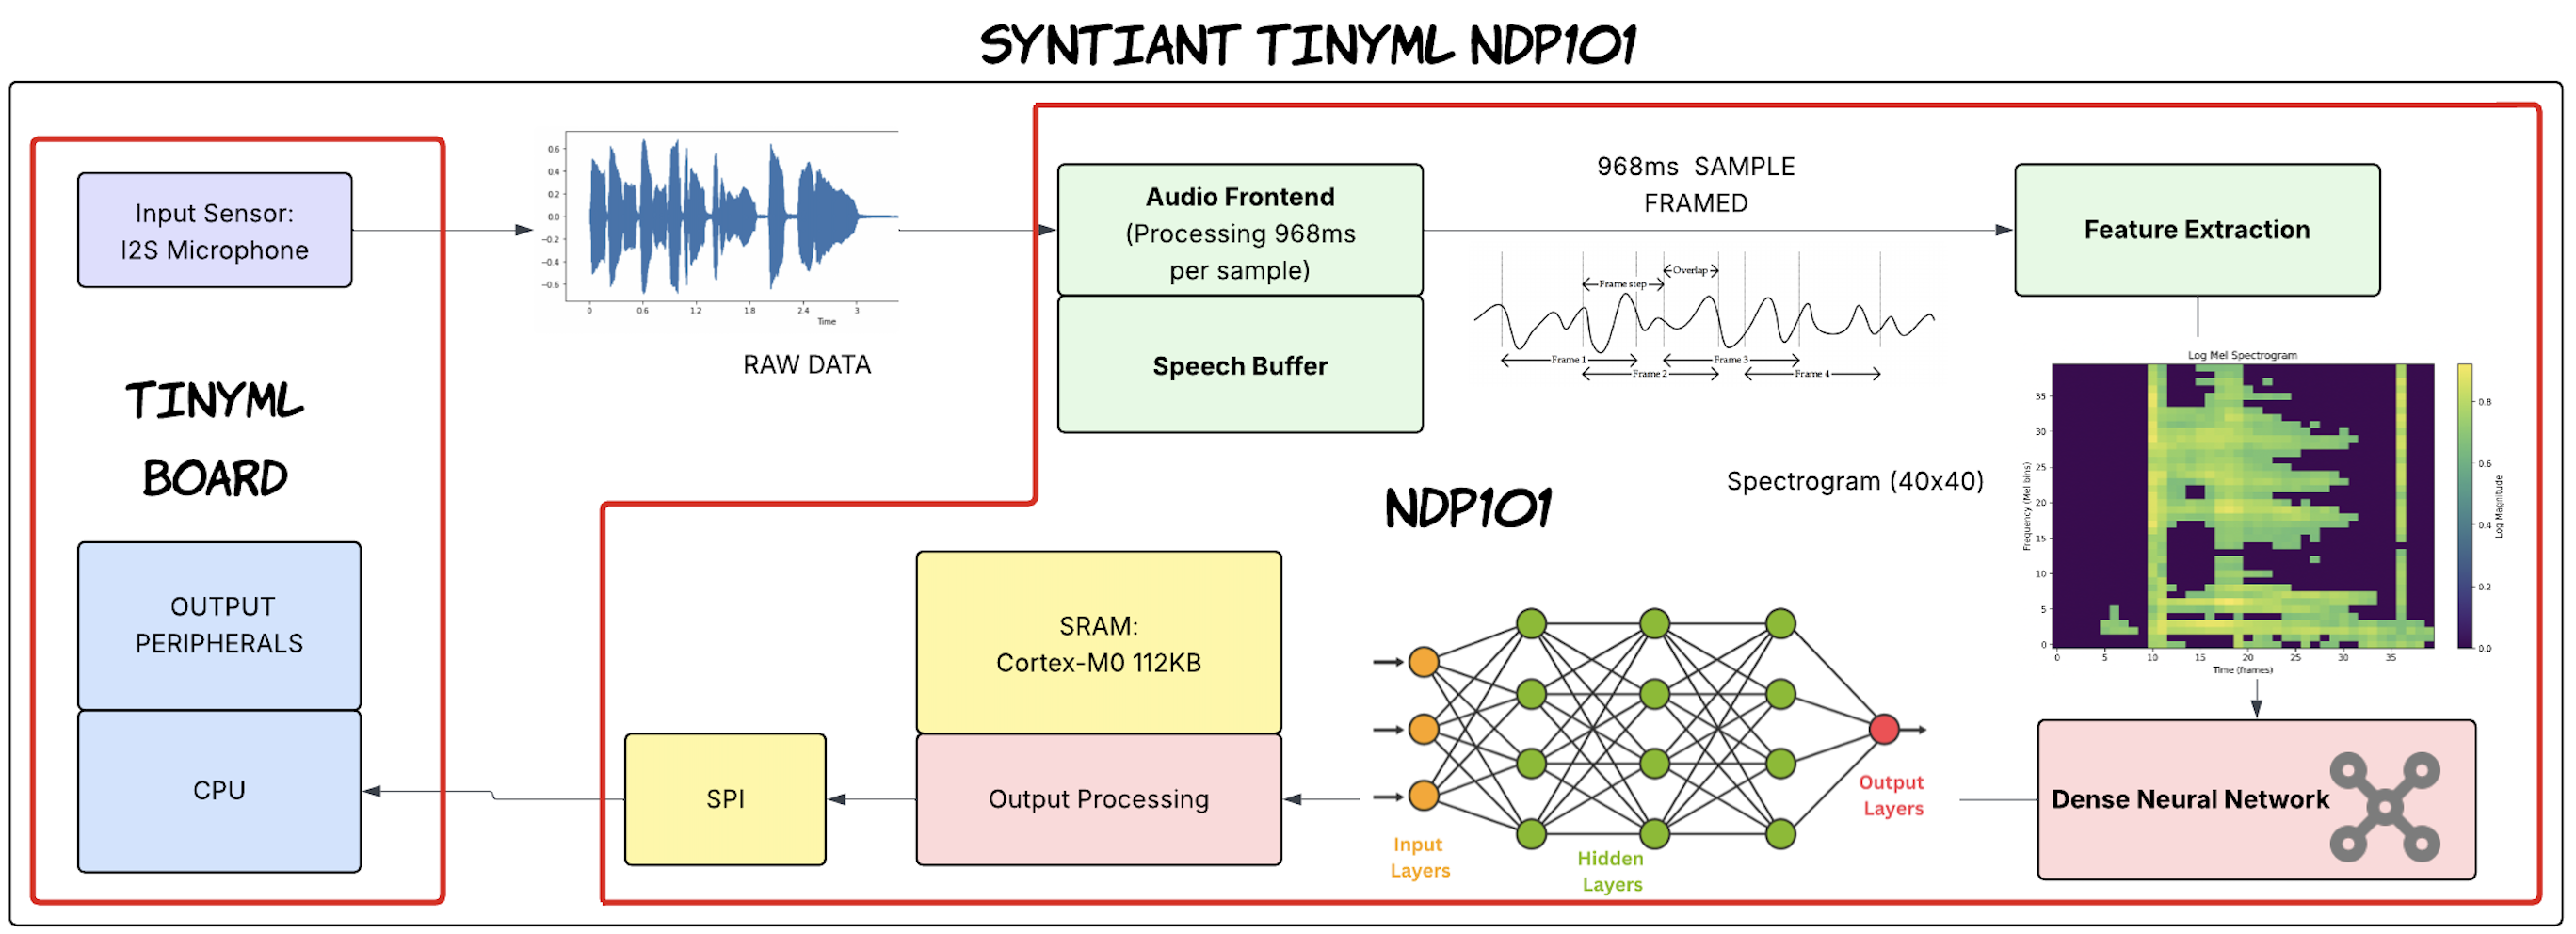
\includegraphics[width=0.9\textwidth]{images/2.01 NDP101 High Level Workflow.png}
        \caption{Syntiant NDP101 High-Level Workflow}
\end{figure}
\newline A typical device behavior involves the use of an already integrated I2S microphone as an input sensor. If the MCU is active, it will always be on, and it will perform a polling behavior. The input is processed by the Audio Front End, which will handle samples of 968ms, while the system feeds a 96KB speech buffer. These samples are given in input to the feature extraction, which will act as MFE Block Processing\cite{syntiant_audio_block}, using log-mel spectrogram. This spectrogram will always have 1600 features, which corresponds to a 40x40 spectrogram image. Then, this generated image is processed by the Dense Neural Network. Although classification is the default behavior, developers can customize how outputs are handled using a custom Arduino IDE code.
\subsection{Device Peripherals}
In addition to the microphone input, the board includes:\newline
• 9 pins: 4 for power supply and 5 for GPIO (general-purpose I/O)\newline
• A Serial Flash Memory (SRAM)\newline
• A micro-SD card slot used for memory extension, which, in this thesis, will not be used. However, for big data storage and the IMU functionality, supported by the device, it is required. It is estimated that with a 32GB card, it will save more than 3 days of uncompressed audio data, using a frequency of 16kHz, and with IMU more than 300 days of 6-axis sensor data using a frequency of 100Hz.\newline
In the following image are shown the peripherals connections on Syntiant NDP101:
\begin{figure}[!h]
    \centering
        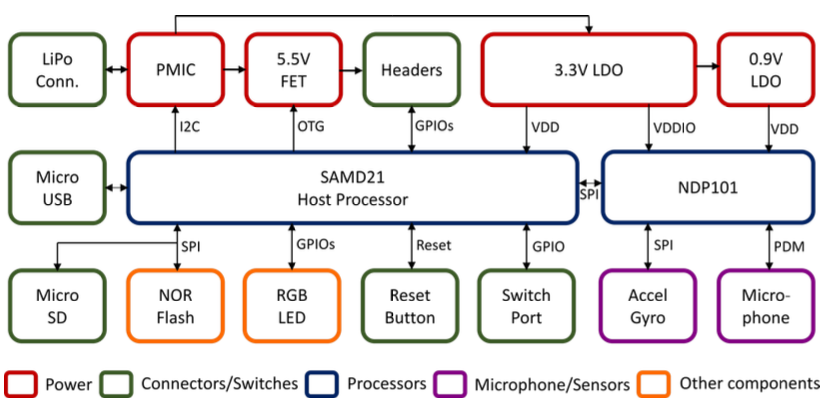
\includegraphics[width=0.9\textwidth]{images/2.02 Design with peripherals.png}
        \caption{Design NDP101 with peripherals}
\end{figure}
\newline Talking about power metrics, according to \cite{analysis_syntiant_performances}, NDP101 is an application using always-on power consumption and it allows the use of audio/voice recognition applications 140$\mu$W. These results compared to others will deliver 20 times more throughput and 200 times less energy per inference. The connection with another MCU is possible with SPI communication; however, without the SDK provided by Syntiant, it is challenging to program the setup of it.
\section{Syntiant Audio Block Processing}
\label{sec:audio}
Edge Impulse reports that Syntiant Audio Block Processing is similar to MFE one\cite{syntiant_audio_block}. Its goal is to extract time and frequency features from a raw audio input. However, the block processing of Syntiant defers a little, because of a noise floor at the end of the computation. The block, which corresponds to the feature extractor, can be viewed as follows:
\begin{figure}[!h]
    \centering
    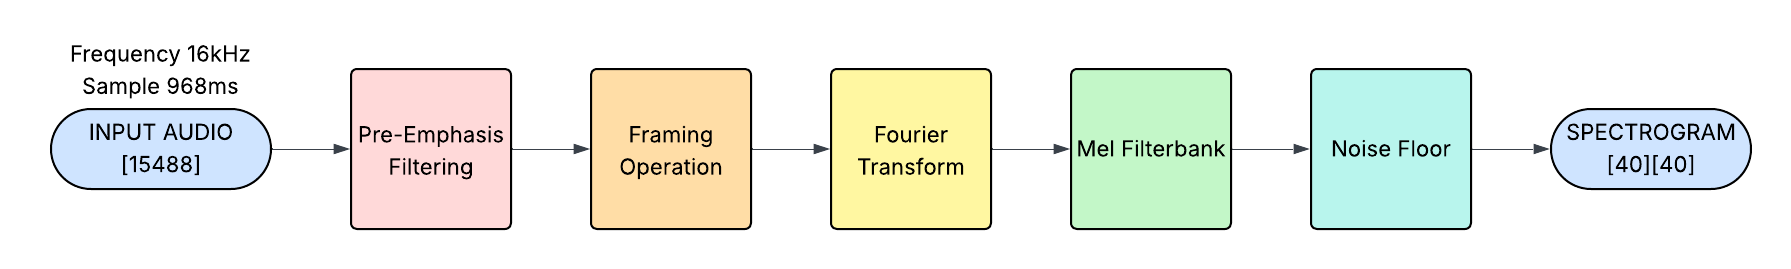
\includegraphics[width=1.0\textwidth]{images/2.03 MFE Block Processing.png}
    \caption{Syntiant Audio Block Processing}
\end{figure}\newline 
1. Input - The frequency of raw data input is at 16kHz and sampling 968ms, it generates 15488 raw data, with short values because the audio sound can go from -$2^{15}$ to $2^{15}-1$. These values come from an implicit ADC (Analog Digital Conversion), using a dual PDM microphone input which interfaces with an I2S interface multiplexed with PDM\cite{PDM_module}. It stands as Pulse Density Modulation, and it reduces the system into a single-bit digital one. This allows signal processing operations to be performed on the audio stream easily, and then the PDM can be modified by the system.  \newline
2. Pre-emphasis filter - This is a high-pass filter that enhances high-frequency components, so the microphone will capture more low-frequency noise and increase high frequencies to make the speech clear. Before this, it is required an audio normalization [-1, 1], generating float values and then applying this high-filter:
\begin{equation}
    y[n]=x[n]-\alpha\cdot x[n-1]
\end{equation}
$\alpha$ consists of a coefficient of filter grade and a standard Syntiant Block set at 0.96875\newline
3. Framing - This audio is split and segmented into small overlapping windows called frames. Each one has an overlap time with each other and on Syntiant device corresponds to 128 floats, considering the size of 512 floats and the stride, how much the start position will move, of 384. In the last frame, a part will overflow the initial buffer, and in that case, the void values are flatted to 0. Considering the input of 15488 samples in a 16kHz frequency:\newline
\begin{equation}
    number\,of\,frames=\frac{input\,size-frame\,size}{frame\,stride}+1=\frac{15488-512}{384}+1=40
\end{equation}
For each frame of the forties computed are performed:\newline
3.1 Windowing - Before performing the Fourier transform, it has to be applied a windowing to reduce spectral leakage in integration, so the following sinusoidal function is used:\newline
\begin{equation}
    0.54-0.46\cdot(\frac{2\pi k}{size-1})
\end{equation}
The size will be 512 and k is an incremental value that goes from 0 up to 511 and k-window is multiplied to the k-position of the array.\newline
3.2 Fast Fourier Transformation (FTT) - This function computes the complex frequency spectrum of a real-valued signal captured in the time domain. It is not required to compute all the DFT domain, because dealing with real value using Hermitian symmetry property with real values, it is required to compute only $\frac{N}{2}+1$ unique complex outputs. 
\begin{equation}
    \begin{cases} 
        X[k]=\sum_{n=0}^{N-1}x[n]\cdot e^{\frac{-2\pi ikn}{N}} & k=0,1,...,\frac{N}{2}\\
        X[l]=\overline{X[k]} & l=N-k
    \end{cases}
\end{equation}
In this case, x[n] is the input signal with n=0,...,N-1, x[n]$\in\mathbb{R}$, i is the imaginary unit, k is the incremental value, and N is the length of the signal (512 values).\newline
3.3 Spectrogram Population - Corresponds to a magnitude computation of the FFT output, obtaining the amplitude spectrum from the complex frequency-domain data. The operation computed the norm of the first half of the Fourier transformation output and saves it in the corresponding size [40x256], the magnitude is computed as follows:
\begin{equation}
    |X[k]|=\sqrt{(Re(X[k]))^2+(Im(X[k]))^2},\,\,k=0,1,...,\frac{N}{2}-1
\end{equation} 
4. Mel-filterbank - After obtaining this matrix, the algorithm applies a mel-filterbank, which is a set of data based on the human perception system via a triangular bandpass filter, making the system more sensitive to low frequencies. It is used mel-scale to obtain this phenomenon because using a logarithmic approach allows better sound recognition.\newline
This implements a K+2 length filter called m, composed of linearly spaced elements, with K as the number of filters.
\begin{equation}
    m[i]=M_{min}+i\cdot\frac{M_{max}-M_{min}}{K+1},\,\,i=0,1,...,K-1
\end{equation}
$M_{min}$ and $M_{max}$ corresponds to the conversion in mel-scale of the minimum and the maximum frequency. Syntiant as default has set the minimum on 0 and the maximum on $\frac{f_s}{2}$. After the information is reconverted back in the frequency scale. The conversion formulas are for Syntiant:
\begin{equation}
    m=1127\cdot log_{10}(1+\frac{h}{700})\,\,\,\,\,\,h=700\cdot 10^{\frac{m}{1127}}-1
\end{equation}
To this scale, a triangular filter for each filter between 1 and K is applied, using bins covering frequencies. The computation of the bins and the triangular function is:
\begin{equation}
    b_i=\lfloor \frac{2\cdot f_i}{f_s}\cdot(N-1)\rfloor\,\,\,\,\,H_k[b]=
    \begin{cases}
        0 & b<b_k-1 or b>b_k+1\\
        \frac{b-b_{k-1}}{b_k-b_{k-1}} & b_{k-1}\leq b \leq b_k\\
        \frac{b_{k+1}-b}{b_{k+1}-b_k} & b_k \leq b \leq b_{k+1}
    \end{cases}
\end{equation}
This computation creates a matrix 40x40, which corresponds to the filterbank filter that will be applied to the magnitudes matrix to obtain a log-mel spectrogram:
\begin{equation}
    L(i,j)=10\cdot log_{10}(\sum_{k=0}^{NUM\_BINS-1}S(i,k)\cdot M(j,k)+\epsilon)\,\,\,i=0,...,N-1\,\,\,j=0,...,F-1\,\,\,\epsilon=10^{-20}
\end{equation}
The computation will generate a 40x40 matrix that will be the form of the image to be fed into the neural network. To the computation is added a small constant error value to avoid log(0) impossible result, L is the log-mel spectrogram, M is the fixed filterbank and S is the spectrogram of the magnitudes\newline
5. Noise Floor - To only maintain audible sound is applied a threshold noise floor flatting all normalized values below 0.65, which should be resized according to the noise floor in decibels of the system which for Syntiant is set to -40dB. The formula to perform this is:
\begin{equation}
    final(i,j)=\frac{L(i,j)-NOISE\,FLOOR}{-NOISE\,FLOOR+12}\,\,\,i,j=0,...,FILTERS
\end{equation}
To be accepted, final(i,j) should be $\geq$ 0.65 and the overall final matrix is the input given to the neural network.
\section{Neural Network Concept}
\subsection{Dense Neural Network (DNN)}
\begin{wrapfigure}{r}{0.4\textwidth}
  \begin{center}
    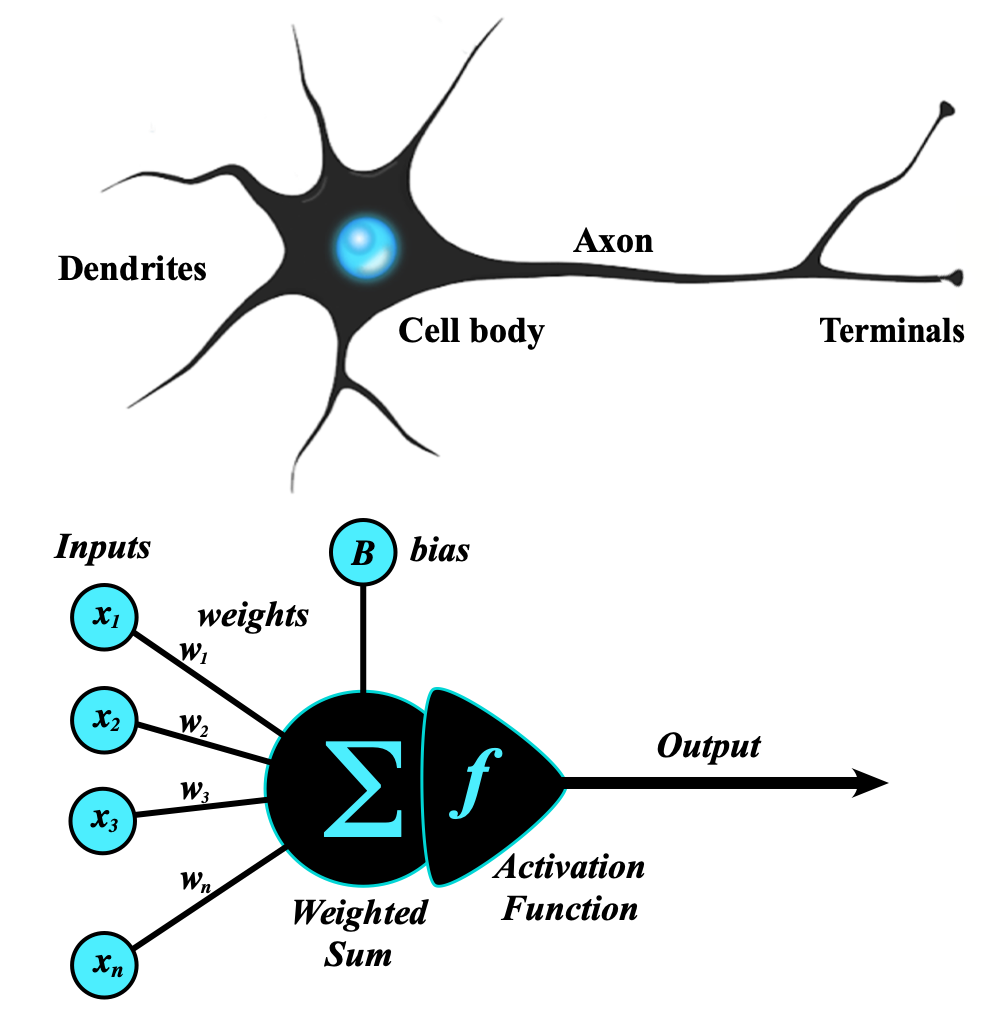
\includegraphics[width=0.38\textwidth]{images/2.04 Neuron.png}
  \end{center}
  \caption{Neuron structure}
\end{wrapfigure}
Neural networks consist of interconnected layers organized in a logical architecture, having inside of each layer a pre-decided number of neurons\cite{neural_network_theory}. These are like nodes that connect two nearby layers. Each receives an input signal and applies to it an activation function, generating an intermediate output that will be passed to the subsequent series of neurons to the other layer. The connections between neurons are weighted, so there are some values associated with the layer that represent the influence of these connections that will modify the input to generate an output. The weights can be adjusted only during the training phase and they characterize the neural network behavior, picking a layer as reference it patterns the connection of each input with each output, generating an allocation in memory equal to "input size$\cdot$ output size". Typically, a bias array is associated to each layer, always modifiable only during training, which performs an adjustment to the output of the neuron. It is like a simple addition, so for each, the array is as big as the output size to have an adjustment value for each output.\newline
To express the neuron mathematically can be defined an input matrix x[N]=[$x_1,...,x_N$$]^T$ as
Nx1, the weights that involve only that output neuron, because it is a big array with size "in\_dimension$\cdot$out\_dimension" and we can express it as matrix w[M]=[$w_1,...,w_M$$]^T$  Mx1, b the bias associated to that neuron, $\phi(\cdot)$ the activation function and y as the output of the neuron, that mathematically will result in:
\begin{equation}
    y=\phi(w^Tx+b)=\phi(\sum_{i=1}^{n}w_ix_i+b)
\end{equation}
More generally, the formula that will represent the output array of a layer will be considering this time the W$\in\mathbb{R}^{O\times N}$ as OxN matrix, the biases b=$[b_1,...,b_O]^T$ as Ox1 matrix and the output as y=$[y_1,...,y_O]^T$ as Ox1 matrix. Results in:
\begin{equation}
    y_i=\phi(Wx+b)=\phi(\sum_{i=1}^{n}w_ijx_i+b_i)\,\,i=1,...,O\rightarrow \begin{cases}
        y_1=\phi(w_{11}x_1+w_{12}x_2+...+w_1Nx_n+b_1)\\
        y_2=\phi(w_{21}x_1+w_{22}x_2+...+w_2Nx_n+b_2)\\
        \dots\\
        y_O=\phi(w_{O1}x_1+w_{O2}x_2+...+w_ONx_n+b_O)\\
    \end{cases}
\end{equation}
The architecture of the neural network is composed of different layers according to their functionality principles. The most notable ones are:\newline
• Input layer: Consists in the input of the system in the case of Syntiant neural network a spectrogram 40x40 flatted into a 1600 features array. This layer is only nominal and it does not perform any computations.\newline 
• Intermediate layer: A neural network can have one or more of these that are between the input and the output layers. The decision of the number of these depends on the memory space and application specifics, but typically more layers equal to a more complex network structure. It is characterized by an activation function typically a ReLU. On the Syntiant NDP101 device, there are 3 intermediate layers each with 256 neurons\newline
• Output layer: Consists in the final output of the network and the output depends on the behavior of the network, if it is a regression-like model it will output inside a neuron a value using an activation ReLU, but if it performs a classification it means it is a multiclass model and in that case is recommended the Softmax activation to identify the probability of belonging in each class. Syntiant devices can have at most 64 neurons as output, with the above neuron configuration.\newline
\begin{center}
    \begin{figure}[!h]
        \centering
        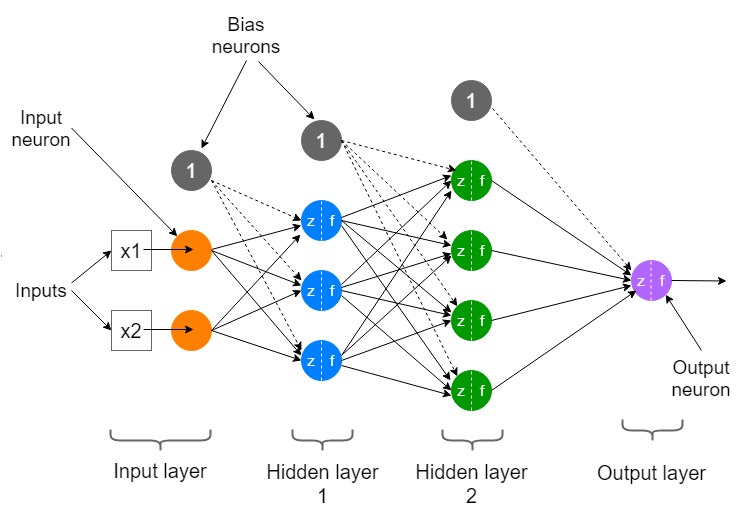
\includegraphics[width=0.75\textwidth]{images/2.05 Neural Network Structure.png}
        \caption{Neural Network Structure}
    \end{figure}
\end{center}
For this thesis, we are interested in only two activation functions, already nominated:\newline
• ReLU (Rectified Linear Unit): Performs a threshold to bring negative values to 0 without touching the positive ones. It is used for its cheapness because it performs a maximum evaluation with 0. In general, the layers rely on this option:\newline
\begin{equation}
    f(x)=max(0,x)
\end{equation}
• Softmax: Used for classification, it converts the output value of the layer in scores with a probability distribution by taking the exponential of each output and normalizing these values by dividing using the sum of all the exponentials. As a counterpart, if summing all the values in the output layer array of the elements, the sum must be 1:\newline
\begin{equation}
    f(x_i)=\frac{e^{x_i}}{\sum_je^{x_j}}
\end{equation}
\subsection{Convolutional Neural Network (CNN)}
A Dense Neural Network has each layer's neurons connected with all the neurons of the subsequent layer. However, there are other neural networks called convolutional, which are more expensive in terms of energy consumption and computationally complex and operate in 2D to apply small filters to scan the input image, which in the case studied would be a spectrogram. It extracts the most prominent features of each area.\newline 
In this section, only the essential notions used in this thesis in the CNN field will be introduced.\newline
The architecture of a standard CNN\cite{introduction_CNN} is composed by:\newline\newline
1. Input Layer - Typically, a CNN receives in input cubes images, with three dimensions (height, width, depth), but in this case, the depth side is not relevant, because the spectrogram is a 1-depth image, requiring only width and height (40x40).\newline
2. Batch Normalization Layer - It applies a normalization to the input to zero-mean and unit-variance. It stabilizes and accelerates training, helping faster learning. The normalization is performed only during training, instead for model usage two trainable parameters are training: one for scaling for a value $\gamma$ and one for shifting for a value $\beta$.\newline
\begin{equation}
    \hat{x}_i = \frac{x_i - \mu_B}{\sqrt{\sigma_B^2 + \epsilon}}, \quad
    y_i = \gamma \cdot \hat{x}_i + \beta
\end{equation}
The parameters are:\newline
• $x_i$ - Input Layer\newline
• $y_i$ - Output Layer\newline
• $\mu_B$ - Mean computation on a subset B. B corresponds to batch being the number of samples condensed in an average behavior minimizing errors\newline
• $\sigma_B$ - Variance computation on a subset B\newline
• $\epsilon$ - Small constant error\newline
\begin{equation}
    \mu_B=\frac{1}{B}\sum_{i=1}^{B}x_i\,\,\,\,\sigma_B^2=\frac{1}{B}\sum_{i=1}^{B}(x_i-\mu_B)^2
\end{equation}
3. Convolutional Layer - It extracts spatial patterns, from the input layer and computes only on that submatrix the neuron operation of DNN, computing a weighted sum using the kernel, which will be composed by weights, adding the bias, and applying a ReLU activation. It may reduce the dimension with downsampling or it may be the same, leaving the job to the max-polling layer, instead of adding channels.\newline
\begin{equation}
    y_{i,j,k}=\sum_{m=0}^{K-1}\sum_{n=0}^{K-1}\sum_{c=0}^{C-1}\omega_{m,n,c,k}\cdot x_{i+m,j+n,c}+b_k
\end{equation}
K corresponds to kernel size, instead of C to the number of channels.\newline
4. Max-polling Layer - On channels, so to the whole image directly, reduces height and width by a window sliding for a pool size and among the values takes the maximum one. It provides spatial invariance, reducing small translations and reducing overfitting by downsampling. The overfitting phenomenon is when the model learns the training data too well, including noise and outliers, rather than underlying patterns that generalize the input data. The phenomenon is seeable if the model performs good training, but fails in validations.
\begin{equation}
    y_{i,j,c}=max_{0<m<P}\,\,max_{o\leq n<P}\,\,x_{i\cdot s+m,\,j\cdot s+n,c}
\end{equation}
P is the polling window size, s is the stride, and max is the maximum value in the pooling region\newline
5. Fully Connected Layer - To recognize the belong to a particular class, it requires at least one FC layer to perform a classification, and it is like in DNN\newline 
\begin{center}
    \begin{figure}[!h]
        \centering
        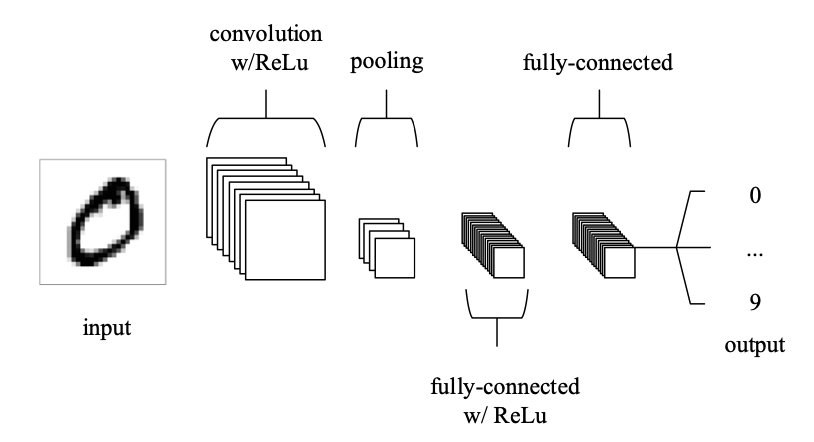
\includegraphics[width=0.8\textwidth]{images/2.06 Convolutional Neural Network.png}
        \caption{Convolutional Neural Network Architecture}
    \end{figure}
\end{center}
\subsection{Neural Network Parameter Performance}
As follows, are listed some notions that will be recalled when talking about models and results:\newline
• Accuracy - Measures the proportion of correct predictions over all predictions:\newline 
\[
\text{Accuracy} = \frac{TP + TN}{TP + TN + FP + FN}
\]
• F1 Score - Harmonic mean of precision and recall, balancing false positives and negatives:\newline 
\[
F1 = \frac{2TP}{2TP + FP + FN}
\]
• Loss - Represents the prediction error:\newline
\[
\mathcal{L} = -\sum y \log(\hat{y})
\]
• AUC (Area Under Curve) - Evaluates classifier performance across all thresholds via ROC curve: \newline 
\[
\text{AUC} = \int_{0}^{1} \text{TPR}(FPR) \, d(\text{FPR})
\]
• EER (Equal Error Rate) - The rate at which the false acceptance rate equals the false rejection rate:\newline
\[
\text{EER} \text{ when } FAR(t) = FRR(t)
\]
• EER Threshold - The decision threshold value at which EER occurs:\newline
\[
t_{\text{EER}} = \arg\min_t |FAR(t) - FRR(t)|
\]
• Cosine Similarity - Measures how similar two vectors are:\newline
\[
\cos(\theta) = \frac{\vec{x} \cdot \vec{y}}{||\vec{x}|| \cdot ||\vec{y}||}
\]

\section{Speaker Verification Approaches}
\label{subsec:sv approaches}
The goal of the thesis is to propose a text-dependent implementation of Syntiant NDP101, leading that each word said by a user has to have a reference sample. From this comes the necessity of having a keyword spotting algorithm to recognize a word and a speaker verification algorithm for extraction of relevant features of the sample and comparison with the word-user reference.\newline\newline
The purpose of speaker verification is to identify if a user is part of a dataset or not. The networks can be trainable with specific user samples, bringing the disadvantage of requiring retraining each time a user is added to the system, so during inference and product release this approach is not recommended. Another solution is choosing a one-time training approach, providing a large dataset of various people. It will generate a feature extraction, which compared with a reference array of equal size can provide the cosine similarity parameter. For application, the second one is the best, but requires more training, a variety amount of data, and a good amount of samples, resulting in a more difficult implementation. Another key difference of the model stays in its text-dependency. If the model is text-dependent, the reference samples of two different words of the same user will be different ones, requiring more memory space allocation with more words required, instead a text-independent approach, which is difficult to achieve without retraining, consists of a memory optimization because the user does not care about saving samples of the words he says, but relies only on his data reference. As a fact, the no-retraining required gives to the model feasibility, instead, text-dependency will provide more accuracy on single words, but will have more memory expenses. It is not our case, but if dealing with a system, not requiring user addition in inference, a solution may be relying on a retraining approach and text-independency. This may be possible only if a large person-dedicated dataset is provided. There are some relevant solutions, to implement a SV model, however, no one is deployable in a Tiny system, except for a d-vector extractor technique, relying on finding patterns in voice before the classification process.\cite{dvector_extractor_TinySV}\newline 

\section{Keyword Spotting Approaches}
\label{subsec:kws approaches}
The goal of the algorithm is to train a neural network to recognize belonging or not to a class output independently from the user. The class can be trained on a sample word or a short phrase. To perform the task efficiently on Syntiant NDP101, it is recommended to develop it using Edge Impulse Framework, which allows a good compression and validation process of the model. The limitations rely on retraining because in performing a text-dependent approach to perform a classification the system should be aware of how a class is composed and characterized. Complex and optimized methods already exist for Embedded Systems, like RNN-based models. This approach uses a Recurrent Neural Network\cite{kws_rnn_based}, which processes a word on character level and, unlike SV models, the various solutions can be deployed for TinyML devices. Edge Impulse, as default, provides directly a model structure compatible with the MCU, because NDP101 architecture is very limited, but it would not rely on a complex dataset and it is a more feasible solution, unlike the SV model.

\newpage